%
% $RCSfile$
%
% Copyright (c) 2005-2006. Christian Heller. All rights reserved.
%
% Permission is granted to copy, distribute and/or modify this document
% under the terms of the GNU Free Documentation License, Version 1.1 or
% any later version published by the Free Software Foundation; with no
% Invariant Sections, with no Front-Cover Texts and with no Back-Cover
% Texts. A copy of the license is included in the section entitled
% "GNU Free Documentation License".
%
% http://www.cybop.net
% - Cybernetics Oriented Programming -
%
% http://www.resmedicinae.org
% - Information in Medicine -
%
% Version: $Revision$ $Date$ $Author$
% Authors: Christian Heller <christian.heller@tuxtax.de>
%

\section{Summary and Outlook}
\label{summary_and_outlook_heading}

This article tried to sum up a much larger scientific work entitled
\emph{Cybernetics Oriented Programming} (CYBOP). In particular, it reflected on
knowledge modelling and its implications on software design. Traditional
concepts were revised with new ideas stemming from various other scientific
disciplines.

\begin{figure}[ht]
    \begin{center}
        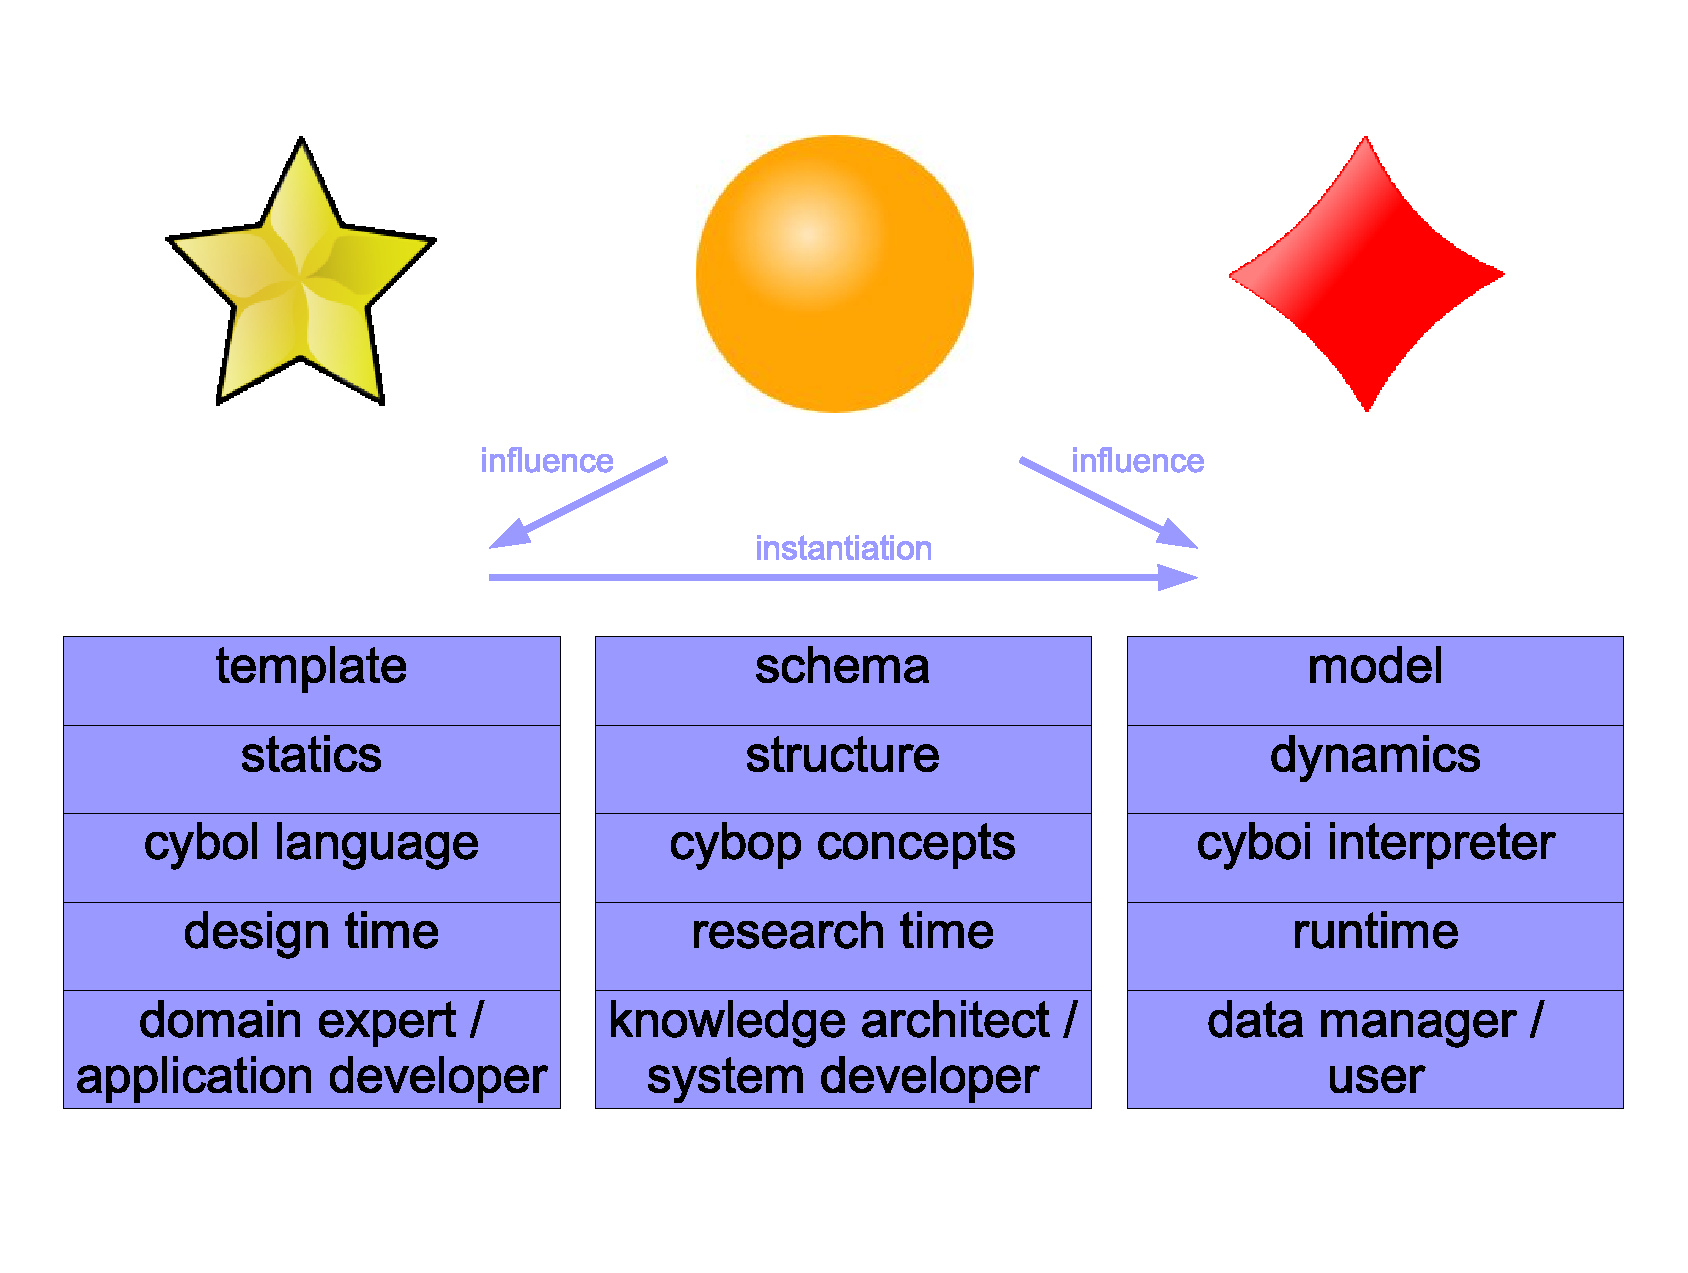
\includegraphics[scale=0.2]{vector/triumvirate.eps}
        \caption{Knowledge Triumvirate}
        \label{triumvirate_figure}
    \end{center}
\end{figure}

The results can be reduced to one illustration: the \emph{Knowledge Triumvirate}
(figure \ref{triumvirate_figure}). Its centrepiece is the new CYBOP knowledge
\emph{Schema} providing a structure to both, knowledge templates and -models.
CYBOI \emph{Models} are the dynamic runtime instances of static design-time
CYBOL \emph{Templates}.

Because all knowledge is stored in tree-form, application systems become much
more flexible than complex class networks as known from OOP. Tree structures
are easy to edit. They allow to better estimate changes caused by new
requirements, because dependencies are obvious. Software maintenance gets
improved, because application developers can focus on pure domain knowledge;
low-level system functionality is provided by CYBOI. CYBOL applications are
therefore not only portable, but represent truely long-life systems.

\begin{figure}[ht]
    \begin{center}
        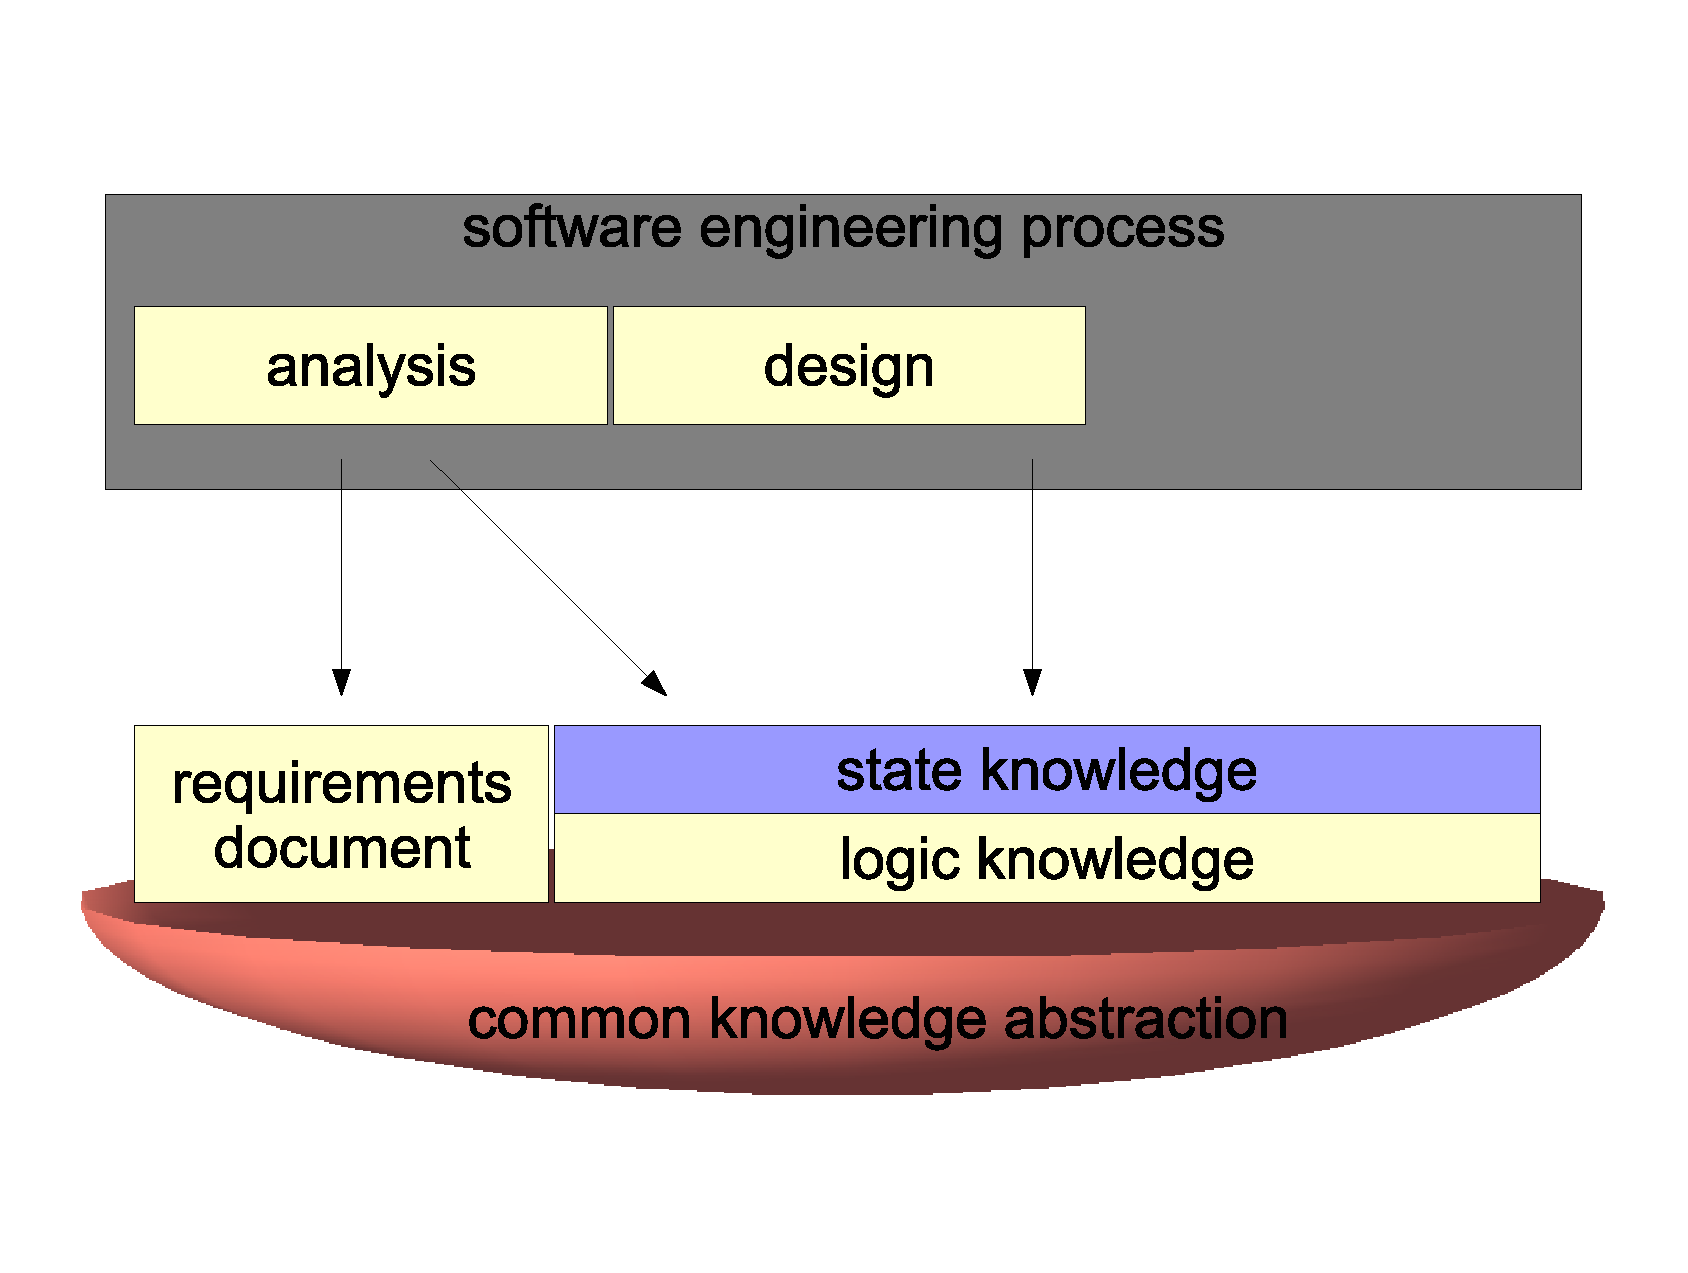
\includegraphics[scale=0.2]{vector/common.eps}
        \caption{Common Knowledge Abstraction}
        \label{common_figure}
    \end{center}
\end{figure}

Although this work does not address the \emph{Software Engineering Process}
(SEP) directly, its results have great effect on it. Section
\ref{abstraction_gaps_heading} pointed out abstraction gaps and multiple
development paradigm switches, happening during a software project's lifetime.
It set out to find a \emph{Common Knowledge Abstraction} for all phases. The
results of this work help overcome \emph{Gap 2} (figure \ref{gaps_figure}).
Since knowledge gets interpreted directly, the formerly needed implementation
phase disappears (figure \ref{common_figure}).

CYBOP applications are capable of communicating universally. CYBOI contains all
necessary mechanisms, so that it suffices to issue a \emph{send}/
\emph{receive} operation with the corresponding language, in a CYBOL template.

Naturally, there are limits to CYBOP. It does not claim to be \emph{the}
approach for all kinds of programming problems, although it thinks to
contribute suitable concepts for business application development. However, its
usability for hardware-close systems with Real Time (RT) requirements is
questionnable, as it cannot guarantee signal execution in time.
